\def\ptitle{ArmoniK : une solution open source pour l'orchestration et la distribution de calculs} % Title
\def\pauthor{Jérôme Gurhem} % Author
\def\pcollaborators{} % Advisors
\def\pteam{Wilfried Kirschenmann} % Team
\def\pinstitute{Aneo, Boulogne-Billancourt, France} % Affiliation
\def\pdate{Jeudi 26 Juin, 2025} % Date
\def\plogo{fig/logo/logo_aneo.png} % Logo of your institution

\pdfobjcompresslevel=0
\documentclass[final]{beamer}
\usepackage[orientation=portrait,size=a0,scale=1.4]{beamerposter}
\usepackage[utf8]{inputenc}
\usepackage[sfdefault]{roboto}
\usepackage[english]{babel}
\usepackage{amsmath, amsthm, amssymb, array, booktabs, grffile, latexsym, tabularx, xspace, hyperref}
\newcolumntype{Z}{>{\centering\arraybackslash}X}
\newcommand{\pphantom}{\textcolor{ta3aluminium}}
\newlength{\columnheight}

\def\purl{\url{https://2025.compas-conference.fr/}}
\def\pdate{\Large Compas, 26 juin 2025} % Date
\def\pmail{\Large Bordeaux ~~~~~~}

\mode<presentation>{\usetheme{COMPAS}}
\title[\ptitle]{\texorpdfstring{\huge \ptitle}{\ptitle}}
\author[\pauthor]{\pauthor\ -\ \padvisors}
\institute[\pinstitute]{\pteam\ -\ \pinstitute}
\date[\pdate]{\pdate}
\setlogo{\plogo}
\setauthorurl{\purl}
\setauthoremail{\pmail}


\usepackage{listings}
\usepackage{tikz}
\usetikzlibrary{positioning, fit, backgrounds, shapes, arrows.meta}

\graphicspath{{./fig/}} % Figures and logos directory
\setlength{\columnheight}{588ex} % Tweak this value if columns are too long/short (should be okay with 588ex)

\definecolor{pykeyword}{rgb}{0.25, 0.3, 0.85}
\definecolor{pycomment}{rgb}{0.0, 0.6, 0.0}
\definecolor{pystring}{rgb}{0.65, 0.1, 0.1}
\definecolor{codebg}{rgb}{0.97, 0.97, 0.97}
\lstdefinestyle{pythonstyle}{
  language=Python,
  basicstyle=\ttfamily\scriptsize,
  keywordstyle=\color{pykeyword}\bfseries,
  commentstyle=\color{pycomment}\itshape,
  stringstyle=\color{pystring},
  backgroundcolor=\color{codebg},
  showstringspaces=false,
  breaklines=true,
  frame=single,
  rulecolor=\color{gray},
  tabsize=2,
  morekeywords={self}, % highlight custom keywords
}

\lstset{style=pythonstyle}



\begin{document}
\begin{frame}[fragile]
    \begin{block}{ArmoniK Positionning in HPC}
    \centering
    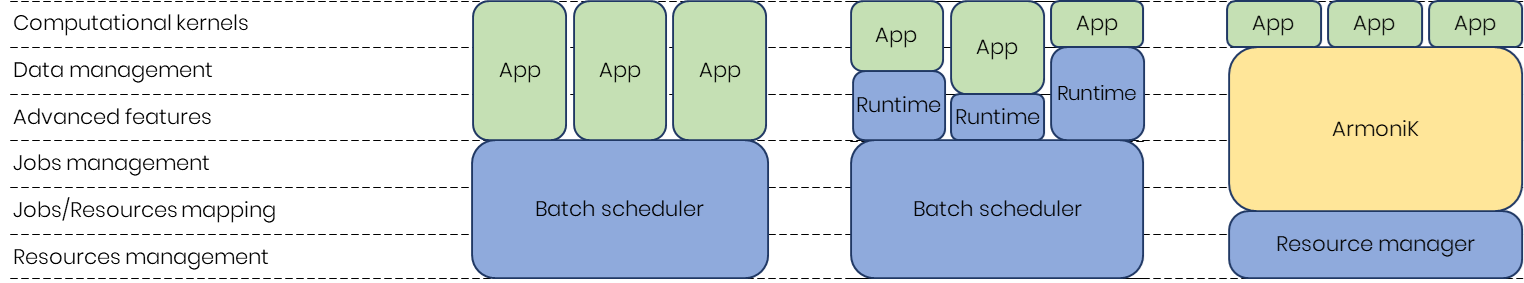
\includegraphics[width=.9\textwidth]{hpc-orchestrators.png}            
    \end{block}
  \begin{columns}
    \begin{column}{.49\textwidth}
      \begin{beamercolorbox}[center,wd=\textwidth]{postercolumn}
        \begin{minipage}[T]{.95\textwidth}
          \parbox[t][\columnheight]{\textwidth}{
            
            \begin{block}{A Serverless Many-Task Computing Platform}
                \begin{alertblock}{Serverless}
                \begin{quote}
                    Cloud service category in which the customer can use different cloud capabilities types
                    without the customer having to provision, deploy and manage either hardware or software
                    resources, other than providing customer application code or providing customer data.
                    \\
                    --- ISO 22123-2:2023
                \end{quote}
                \end{alertblock}
                \begin{alertblock}{Many-Task Computing}
                \begin{quote}
                    Approach that aims to bridge the gap between High-Perfomance Computing and High-Throughput Computing.
                    \\
                    --- Wikipedia
                \end{quote}
                \end{alertblock}         
            \end{block}
            
            % \begin{block}{Simplified Architecture}
            % \centering
            % 
\begin{tikzpicture}[
    font=\sffamily,
    box/.style={
      draw,
      fill=blue!10,
      minimum width=4em,
      minimum height=2em,
      align=center
    },
    object/.style={
      tape,
      tape bend top=none,
      tape bend height=1em,
      fill=purple!10,
      draw,
    },
    database/.style={
      cylinder,
      fill=purple!10,
      aspect=0.25,
      draw,
      shape border rotate=90
    },
    queue/.style={
      cylinder,
      fill=purple!10,
      aspect=0.25,
      draw,
    },
    container/.style={
      draw,
      thick,
      label={[yshift=-3.5ex]north:#1},
      inner sep=4ex,
      rounded corners=4pt
    },
    bg container/.style={
      draw,
      inner sep=0pt,
      fit=#1,
      rounded corners=4pt
  },
  arrow/.style={-Stealth},
  biarrow/.style={Stealth-Stealth},
]

\newcommand{\dashedLineWithDots}[2]{%
  \fill[gray] (#1) circle (2pt);
  \draw[dashed, color=gray, bend right, thick] (#1) -- (#2);
  \fill[gray] (#2) circle (2pt);
}

% Compute Plane
\node[box] (agent1) {Agent};
\node[box, below=0.5cm of agent1] (worker1) {Worker};
\draw[biarrow] (agent1) -- (worker1);

\node[box, right=4cm of agent1] (agent2) {Agent};
\node[box, below=0.5cm of agent2] (worker2) {Worker};
\draw[biarrow] (agent2) -- (worker2);

% Fit Instances
\node[container={Instance}, fit=(agent1)(worker1)] (inst1) {};
\node[container={Instance}, fit=(agent2)(worker2)] (inst2) {};

% Partition
\node[container={Partition}, fit=(inst1)(inst2)] (partition) {};

% Compute Plane
\node[container={Compute Plane}, fit=(partition)] (computeplane) {};

% Control Plane
\node[box, below=1.3cm of computeplane, xshift=2em] (submitter) {Submitter};
\node[box, right=1cm of submitter] (logs) {Logs};
\node[box, right=1cm of logs] (metrics) {Metrics};
\node[container={Control Plane}, fit=(submitter)(metrics)(logs)] (controlplane) {};

% Storage
\node[queue, below left=2cm of controlplane] (queue) {Queue};
\node[object, right=1cm of queue] (object) {Object};
\node[database, right=1cm of object] (database) {Database};
\node[container={Storage}, fit=(queue)(object)(database)] (storage) {};

% Arrows
\draw[arrow, bend right] (agent1.west) to (storage);
\draw[arrow, bend right] (agent2.west) to (storage);
\draw[arrow] (submitter) -- (storage);
\draw[arrow] (metrics) -- (database);

% Dotted line between partition and metrics
\dashedLineWithDots{[xshift=-4em]partition.south east}{metrics.north}

% Fill background of each container
\begin{pgfonlayer}{background}
  \node[bg container={(computeplane)}, fill=gray!10] {};
  \node[bg container={(partition)}, fill=yellow!20] {};
  \node[bg container={(inst1)}, fill=green!10] {};
  \node[bg container={(inst2)}, fill=green!10] {};
  \node[bg container={(controlplane)}, fill=gray!10] {};
  \node[bg container={(storage)}, fill=blue!10] {};
\end{pgfonlayer}

\end{tikzpicture}
            % \end{block}

            \begin{block}{Task Definition in ArmoniK}
            \lstinputlisting[language=Python]{task-based-programming.py}
            \end{block}

            \begin{block}{Dynamic Graph}
            \begin{itemize}
                \item Dependency graph is not fully known when scheduling starts
                \item Submissions can happen anytime
                \item Tasks can submit new tasks
                \item Tasks can delegate the production of their output to their new tasks
            \end{itemize}
            \begin{columns}[T]
            \begin{column}{0.3\textwidth}
                \centering
                \vspace{1cm}
                \vfill
                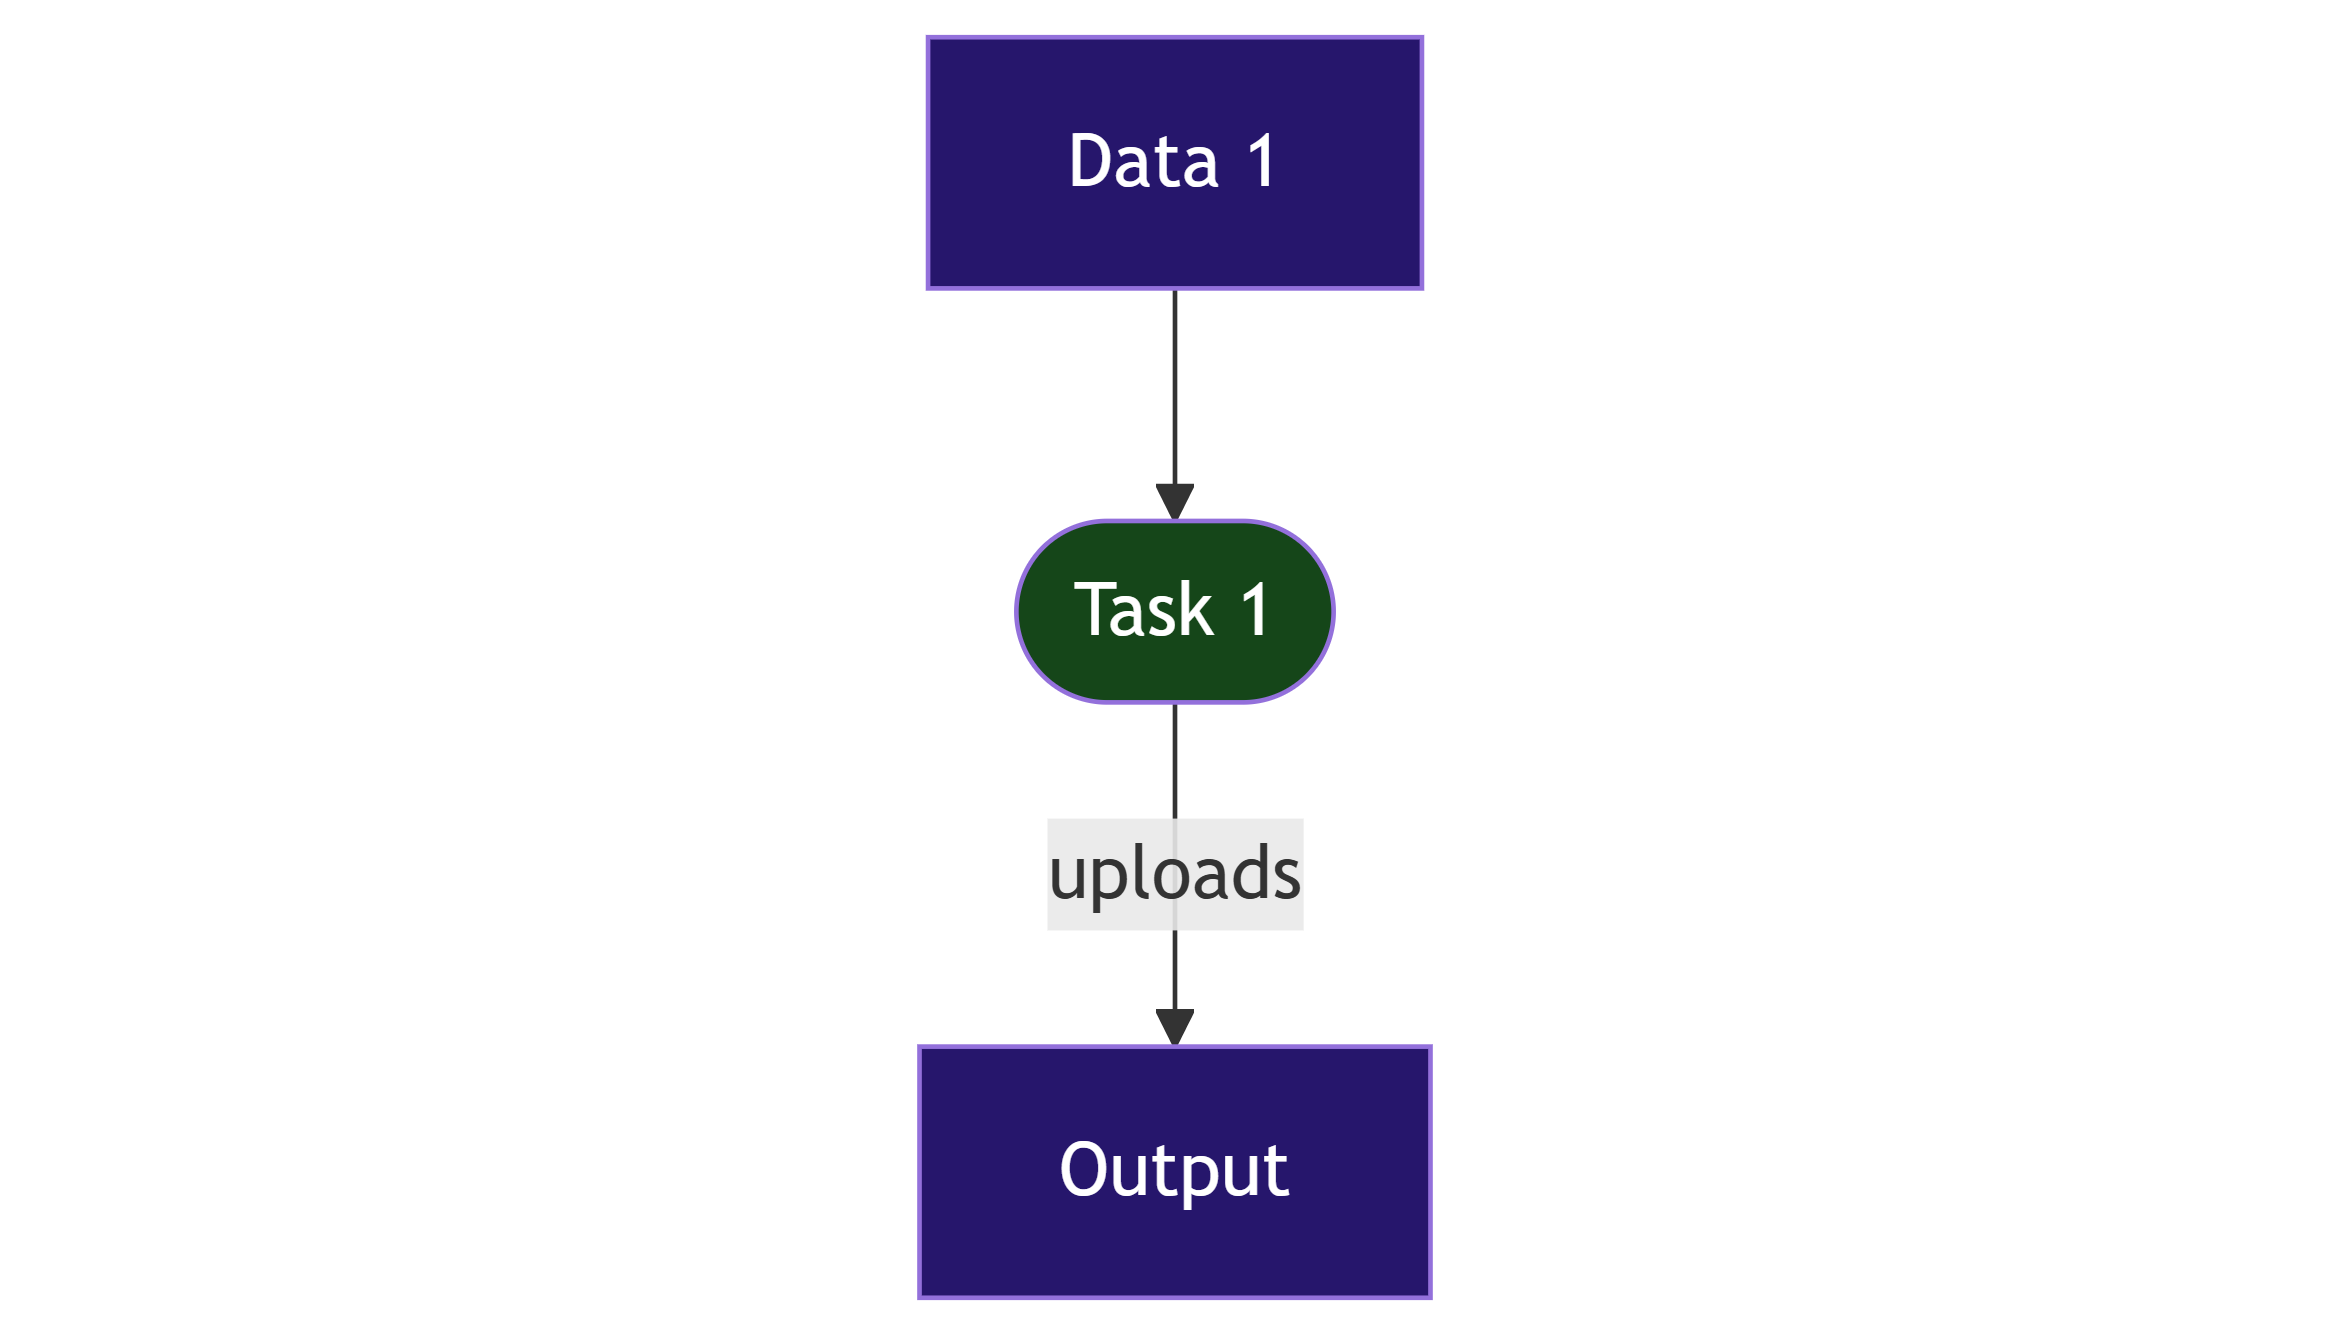
\includegraphics[width=0.95\textwidth]{mermaid-dynamic-part1.png}
            \end{column}
            \begin{column}{0.05\textwidth}
                \centering
                \vspace{1.7cm}
                \vfill
                $\Rightarrow$
            \end{column}
            \begin{column}{0.65\textwidth}
                \centering
                \footnotesize
                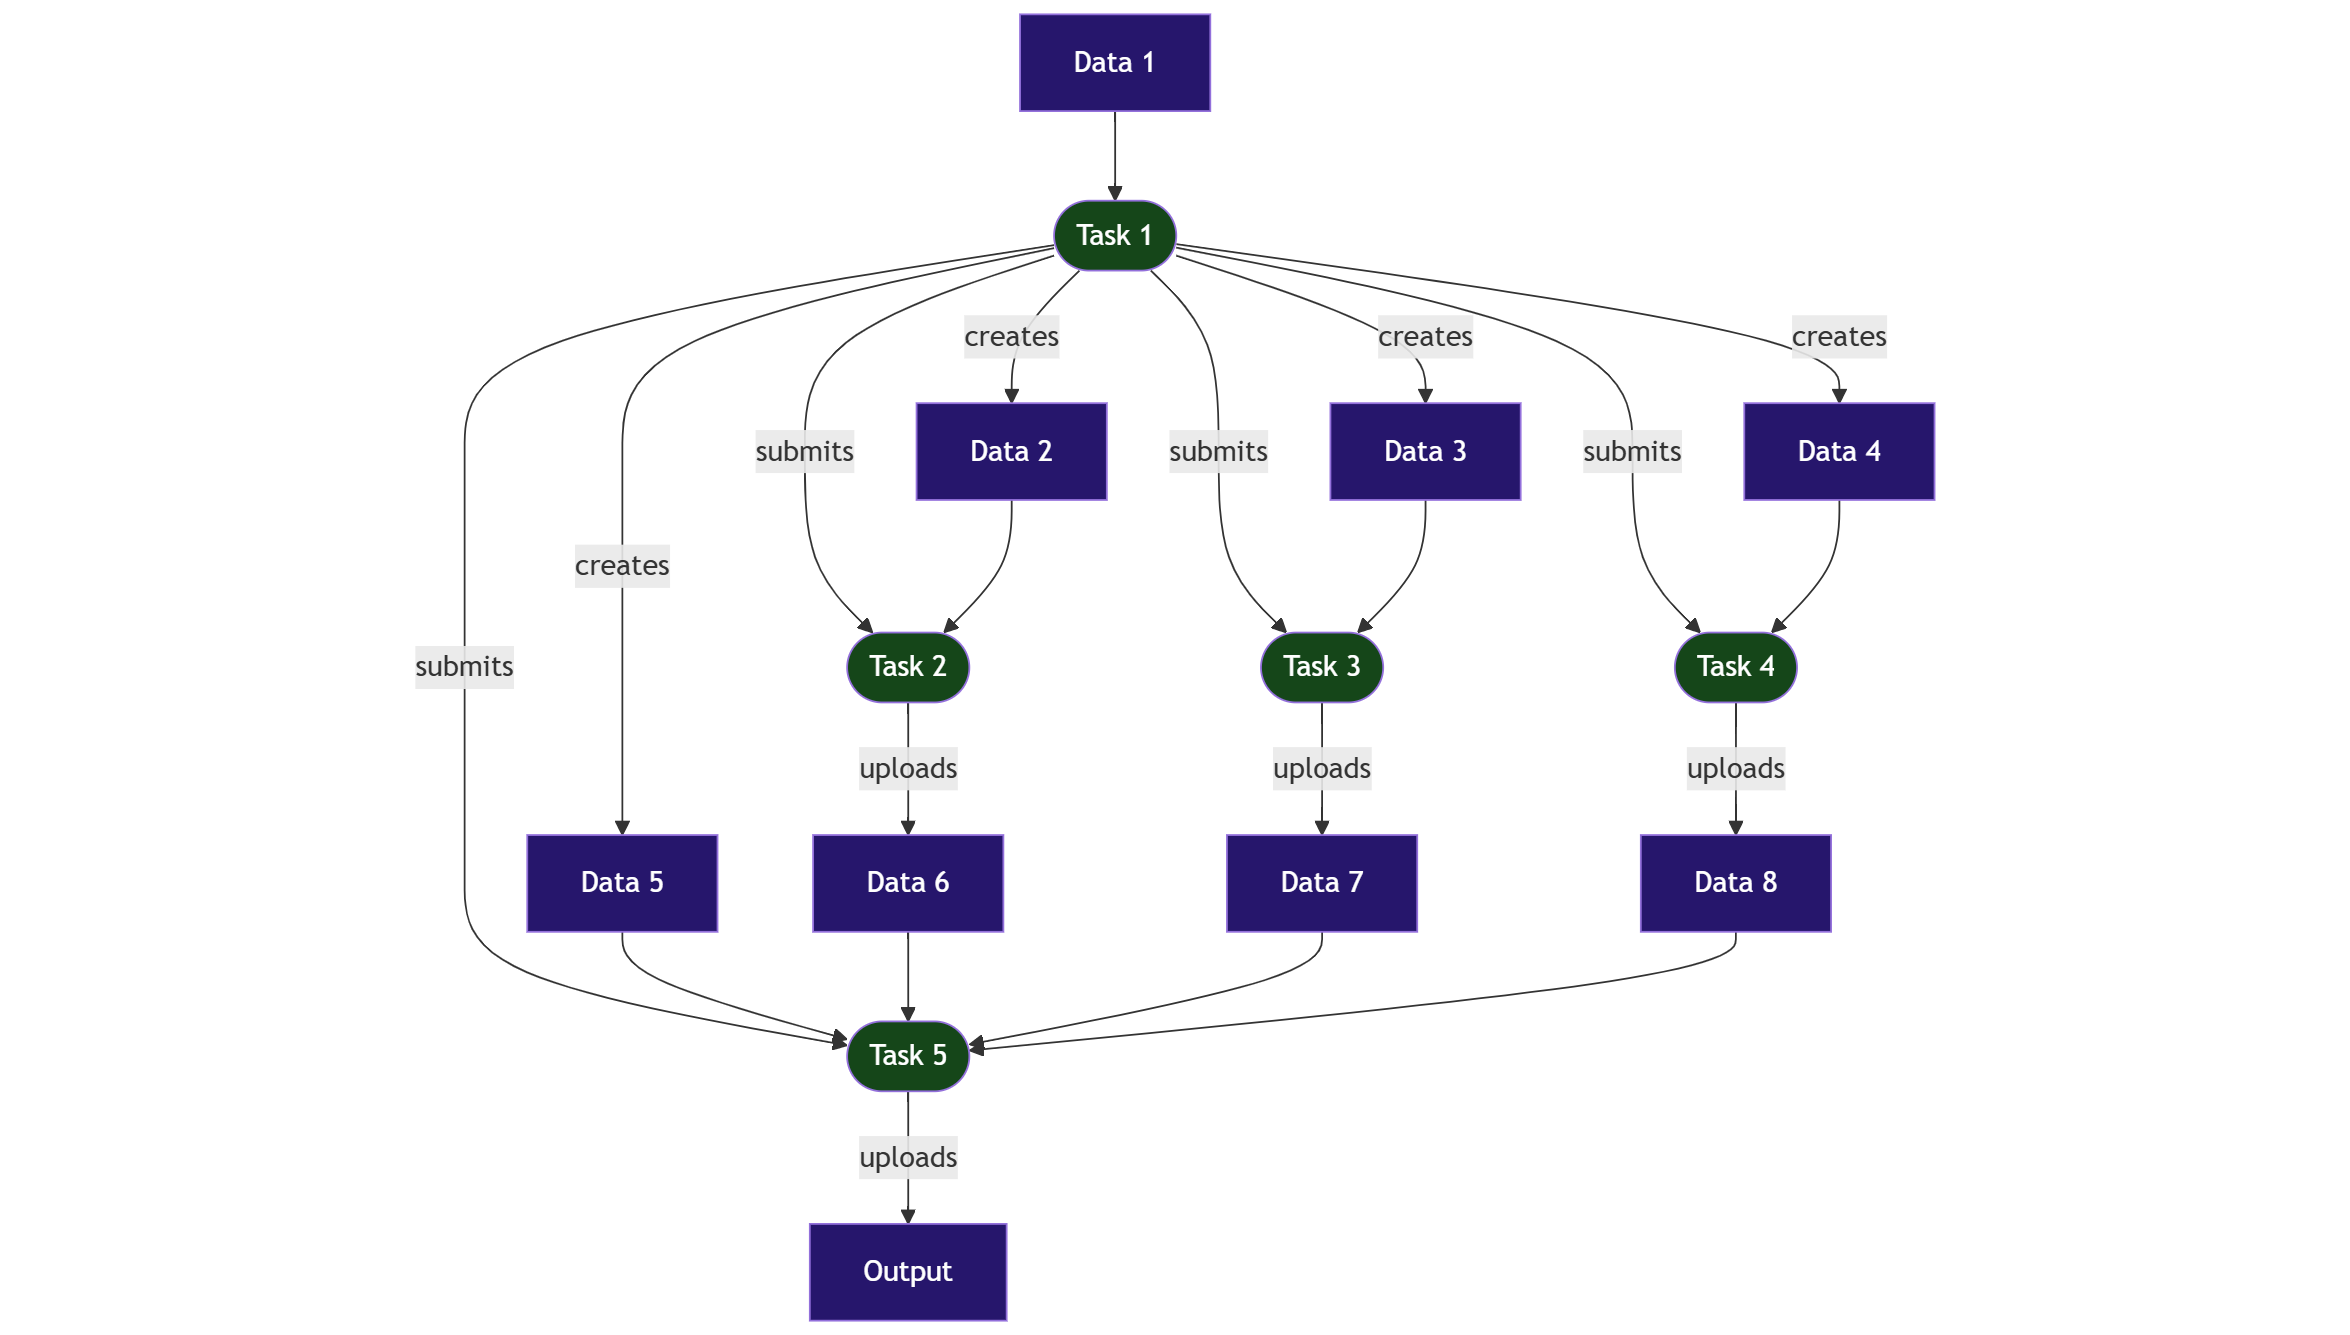
\includegraphics[width=0.95\textwidth]{mermaid-dynamic-part2.png}
            \end{column}
            \end{columns}
            \end{block}

            \begin{block}{Dynamic Graph Example}
            \lstinputlisting[language=Python]{subtasking.py}
            \end{block}

          }
        \end{minipage}
      \end{beamercolorbox}
    \end{column}
    \begin{column}{.49\textwidth}
      \begin{beamercolorbox}[center,wd=\textwidth]{postercolumn}
        \begin{minipage}[T]{.95\textwidth}
          \parbox[t][\columnheight]{\textwidth}{
            
            \begin{block}{Task-based Programming in ArmoniK}
            
                \begin{itemize}
                \item Expression of complex data-driven dependencies
                \item ArmoniK's \textbf{distributed scheduler} responsible for:
                \begin{itemize}
                    \item Task distribution and load balancing
                    \item Dependency resolution
                    \item Tasks execution
                    \item Data management (overlapping, prefetching, and checkpointing)
                \end{itemize}
                \end{itemize}
            \end{block}
            


            \begin{block}{Computations/Comm Overlapping}
                \begin{itemize}
                \item ArmoniK is responsible for tasks input and output data management
                \item Allows for automatic communication + scheduling/task execution overlapping
                \item Automatic Uncoordinated Checkpointing
                \item Data communications through global storage
                \end{itemize}
                \vspace{3ex}
                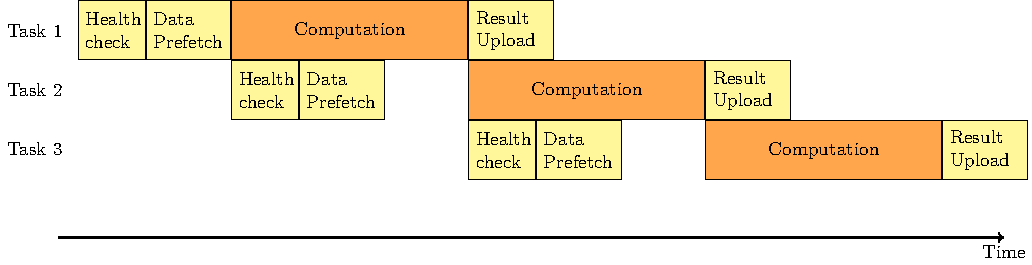
\includegraphics[width=0.8\textwidth]{armonik_pipelining.pdf}
            \end{block}


            \begin{block}{Main features}
                \begin{itemize}
                \item \textbf{Observability}: Understanding of the internal state of a system based solely on its external outputs
                \begin{itemize}
                    \item GUIs, CLIs, monitoring APIs, metrics, logs, and traces
                \end{itemize}
                \item \textbf{Portability}: Effort to transfer an application from one environment to another
                \begin{itemize}
                    \item Officially supported languages: C\#, C++, Python, Rust, Java, and JavaScript
                    \item Tasks on different architectures (x86, ARM, GPU, Linux, Windows), applications, environments
                \end{itemize}
                \item \textbf{Fault Tolerance}: Ability to continue functioning without interruption when one or more nodes fail
                \begin{itemize}
                    \item Allow support for preemptible computing resources
                    \item Error management at the task level
                \end{itemize}
                \item \textbf{Malleability}: Dynamic reconfiguration of the number of allocated resources during execution without interruption
                \item \textbf{Resource Sharing}: Share resources between applications to execute as many as possible at the same
                \item \textbf{Modularity}: Modules can be swapped without modifying ArmoniK's code to suit user neeeds and constraints
                \end{itemize}
            \end{block}

          }
        \end{minipage}
      \end{beamercolorbox}
    \end{column}
  \end{columns}
  \vskip1ex
\end{frame}
\end{document}